\documentclass[aspectratio=169,10pt]{beamer}
\usepackage[utf8]{inputenc}
\usepackage[T1]{fontenc}
\usepackage[spanish, es-tabla]{babel}
\usepackage{amsmath, amsfonts, amssymb, amsthm}
\usepackage{graphicx}
\usepackage{booktabs}
\usepackage{tikz}
\usepackage{listings}
\usepackage[most]{tcolorbox}
\usepackage{float}
\usepackage{hyperref}

\usetikzlibrary{arrows.meta, positioning, automata, trees}
\usetikzlibrary{babel}

\usetheme{Madrid}

\usecolortheme{default}

\setbeamertemplate{navigation symbols}{}

% Número de diapositiva
\setbeamertemplate{footline}{
    \leavevmode%
    \hbox{%
        \begin{beamercolorbox}[
            wd=.85\paperwidth,
            ht=2.5ex,
            dp=1ex,
            leftskip=1em
        ]{author in head/foot}
            \textbf{Ricardo López Ramírez}
        \end{beamercolorbox}%
        \begin{beamercolorbox}[
            wd=.15\paperwidth,
            ht=2.5ex,
            dp=1ex,
            center
        ]{date in head/foot}
            \insertframenumber/\inserttotalframenumber
        \end{beamercolorbox}%
    }
}

% ------------------------------------------------
% INFORMACIÓN DE LA PRESENTACIÓN
% ------------------------------------------------

\title[
    Certificaciones DBA
]{
    Database Administrator
}

\subtitle{
    Certificaciones DBA
}

\author{
    Ricardo López Ramírez
}

\institute{
    Facultad de Estudios Superiores Acatlán \\
    Matemáticas Aplicadas y Computación
}

\date{\today}


% Bloque de ejercicio
\newtcolorbox{ejercicio}[1][]{
    enhanced,
    sharp corners,
    boxrule=0pt,
    leftrule=4pt,
    colframe=gray!50!black,
    colback=gray!5!white,
    title=#1,
    fonttitle=\bfseries
}

% Bloque de alerta
\newtcolorbox{alerta}[1][]{
    enhanced,
    sharp corners,
    boxrule=0pt,
    leftrule=4pt,
    colframe=red!60!black,
    colback=red!5!white,
    title=#1,
    fonttitle=\bfseries
}

% Bloque de nota
\newtcolorbox{nota}[1][]{
    enhanced,
    sharp corners,
    boxrule=0pt,
    leftrule=4pt,
    colframe=orange!70!black,
    colback=yellow!5!white,
    title=#1,
    fonttitle=\bfseries
}


\begin{document}

\begin{frame}
    \titlepage
\end{frame}


\begin{frame}{Contenido}
    \tableofcontents
\end{frame}



\section{Introducción}

\begin{frame}{Las certificaciones de Administración de Bases de Datos}

    \begin{block}{}
        Un \textbf{Database Administrator (DBA)} es el profesional
        encargado de administrar, mantener, proteger y optimizar
        los sistemas de bases de datos de una organización.
    \end{block}

    \vspace{1mm}

    Actualmente, las empresas tecnológicas como Microsoft, Oracle, IBM, 
    Amazon Web Services(AWS) y Google ofrecen certificaciones de bases de datos
    Estas certificaciones pueden incluir cursos de preparación, laboratorios prácticos y exámenes que 
    permiten validar los conocimientos técnicos de los candidatos.

    \vspace{1mm}

    En esta investigación se analizarán cinco certificaciones relacionadas con la administración de bases de datos, considerando tanto alternativas disponibles en México como certificaciones con reconocimiento internacional.

\end{frame}


\section{Microsoft Certified: Azure Fundamentals}

\begin{frame}{Microsoft Certified: Azure Fundamentals}

    \begin{columns}[T]

        \column{0.60\textwidth}

        \begin{block}{Microsoft Certified: Azure Fundamentals (AZ-900)}
            \begin{itemize}
                \item Producto: Microsoft Azure, plataforma de servicios de computación en la nube.
                \item Empresa: Microsoft Corporation es una empresa tecnológica estadounidense dedicada al software, servicios en la nube, inteligencia artificial y soluciones empresariales.
                \item cursos previos: Introducción a la infraestructura en la nube (AZ-900T00-A), duración de 1 día; el material autodirigido de Microsoft Learn es gratuito.
                \item Certificación: Microsoft Certified: Azure Fundamentals (AZ-900), examen de 45 minutos y costo aproximado de US \( \mathdollar 84\) en la región mostrada por Microsoft.
            \end{itemize}
        \end{block}

    \end{columns}

\end{frame}

\section{Microsoft Azure}

\begin{frame}{Microsoft Azure}

       \begin{columns}[T]

        % Imagen izquierda
        \column{0.48\textwidth}
        \centering
        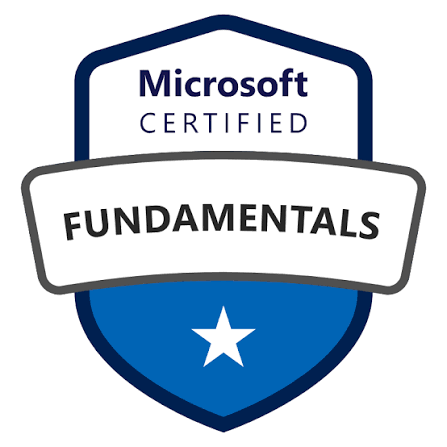
\includegraphics[width=0.75\textwidth]{../../Archivos/Imagenes_Logos/Microsoft_1.png}

        \vspace{0.2cm}

        

        % Imagen derecha
        \column{0.48\textwidth}
        \centering
        
\includegraphics[width=0.75\textwidth]{../../Archivos/Imagenes_Logos/Microsoft_2.png}

        \vspace{0.2cm}

       

    \end{columns}

\end{frame}


\section{AWS Certified Cloud Practitioner}

\begin{frame}{AWS Certified Cloud Practitioner}

    \begin{columns}[T]

        \column{0.65\textwidth}

        \begin{block}{Amazon Web Services  AWS Certified Cloud Practitioner}
            \begin{itemize}
                \item Producto: Amazon Web Services (AWS), plataforma de computación en la nube.
                \item Empresa: Amazon Web Services es una división de Amazon especializada en infraestructura, almacenamiento, bases de datos, inteligencia artificial y servicios cloud.
                \item Cursos previos: AWS Cloud Practitioner Essentials, curso digital autoguiado de 6 horas y gratuito; AWS también ofrece un plan de aprendizaje específico para la certificación.
                \item Certificación: AWS Certified Cloud Practitioner, examen de 90 minutos, 65 preguntas y costo de US\(\mathdollar 100\); tiene una vigencia de tres años.
            \end{itemize} 
        \end{block}

    \end{columns}

\end{frame}

\section{Amazon Web Services}

\begin{frame}{Amazon Web Services}

       \begin{columns}[T]

        % Imagen izquierda
        \column{0.48\textwidth}
        \centering
        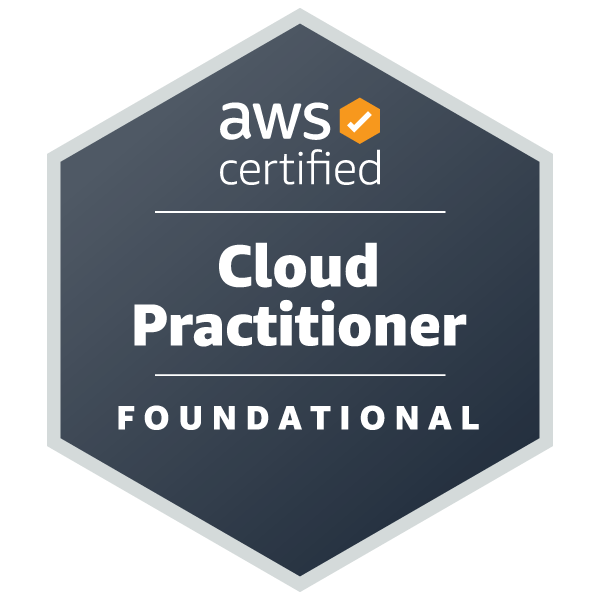
\includegraphics[width=0.75\textwidth]{../../Archivos/Imagenes_Logos/AWS_1.png}

        \vspace{0.2cm}

        

        % Imagen derecha
        \column{0.48\textwidth}
        \centering
        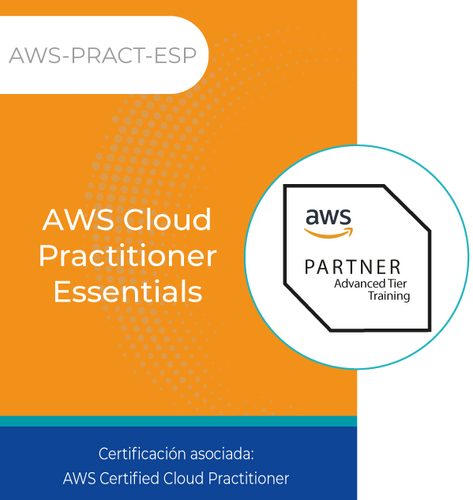
\includegraphics[width=0.75\textwidth]{../../Archivos/Imagenes_Logos/AWS_2.png}

        \vspace{0.2cm}

        

    \end{columns}

\end{frame}


\section{Google Cloud Associate Cloud Engineer}

\begin{frame}{Google Cloud Associate Cloud Engineer}

    \begin{columns}[T]

        \column{0.65\textwidth}

        \begin{block}{Associate Cloud Enginee}
            \begin{itemize}
                \item Producto: Google Cloud, plataforma de servicios de computación y datos en la nube.
                \item Empresa: Google LLC es una empresa tecnológica estadounidense perteneciente a Alphabet, especializada en servicios de Internet, software, inteligencia artificial y computación en la nube.
                \item Cursos previos: Google recomienda el Cloud Engineer Learning Plan, que incluye cursos, laboratorios y recursos prácticos; Google Skills tiene suscripciones desde US\(\mathdollar29\) mensuales.
                \item Certificación: Associate Cloud Engineer; examen de 2 horas, costo de US\(\mathdollar125\) más impuestos, sin requisitos formales y con vigencia de tres años.
            \end{itemize} 
        \end{block}

    \end{columns}

\end{frame}


\section{Google Cloud}

\begin{frame}{Google Cloud}

       \begin{columns}[T]

        % Imagen izquierda
        \column{0.48\textwidth}
        \centering
        
\includegraphics[width=0.75\textwidth]{../../Archivos/Imagenes_Logos/Google_1.png}

        \vspace{0.2cm}

       

        % Imagen derecha
        \column{0.48\textwidth}
        \centering
        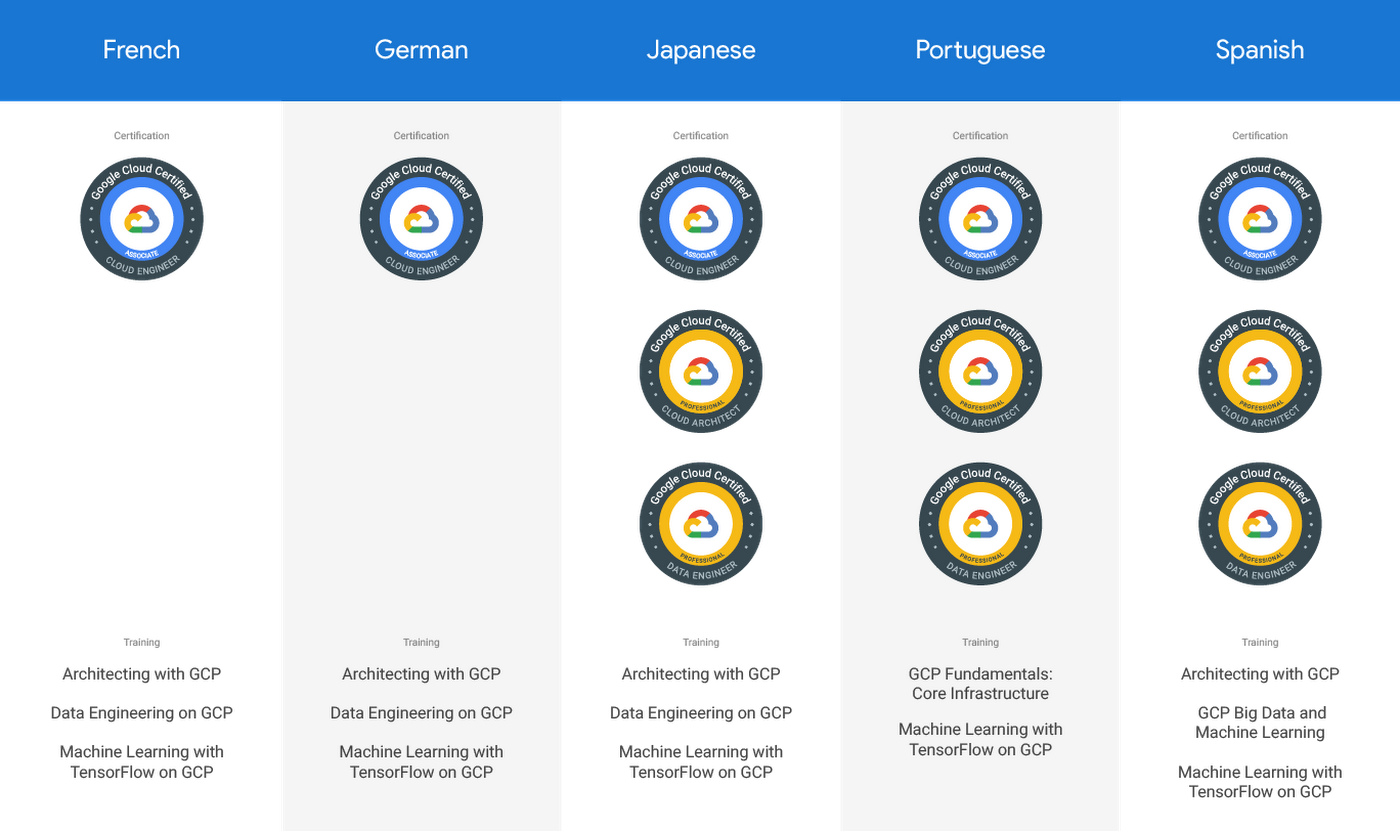
\includegraphics[width=0.75\textwidth]{../../Archivos/Imagenes_Logos/Google_2.png}

        \vspace{0.2cm}

       

    \end{columns}

\end{frame}


\section{Cisco Certified Network Associate (CCNA)}

\begin{frame}{Cisco Certified Network Associate (CCNA)}

    \begin{columns}[T]

        \column{0.65\textwidth}

        \begin{block}{Cisco}
            \begin{itemize}
                \item Producto: Cisco Networking, soluciones de redes, seguridad y automatización.
                \item Empresa: Cisco Systems, Inc. es una empresa estadounidense especializada en redes, ciberseguridad, comunicaciones y tecnologías de infraestructura.
                \item Cursos previos: Implementing and Administering Cisco Solutions (CCNA); la modalidad dirigida dura 5 días de clase más 3 días de autoestudio. Cisco también ofrece recursos introductorios gratuitos mediante Networking Academy.
                \item Certificación: Cisco Certified Network Associate (CCNA 200-301), examen de 120 minutos y costo de US \(\mathdollar300\) según la página oficial consultada.
            \end{itemize} 
        \end{block}

    \end{columns}

\end{frame}

\section{Cisco}

\begin{frame}{Cisco}

       \begin{columns}[T]

        % Imagen izquierda
        \column{0.48\textwidth}
        \centering
        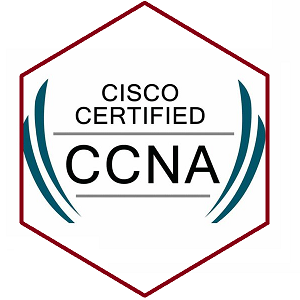
\includegraphics[width=0.75\textwidth]{../../Archivos/Imagenes_Logos/Cisco_1.png}

        \vspace{0.2cm}

        

        % Imagen derecha
        \column{0.48\textwidth}
        \centering
        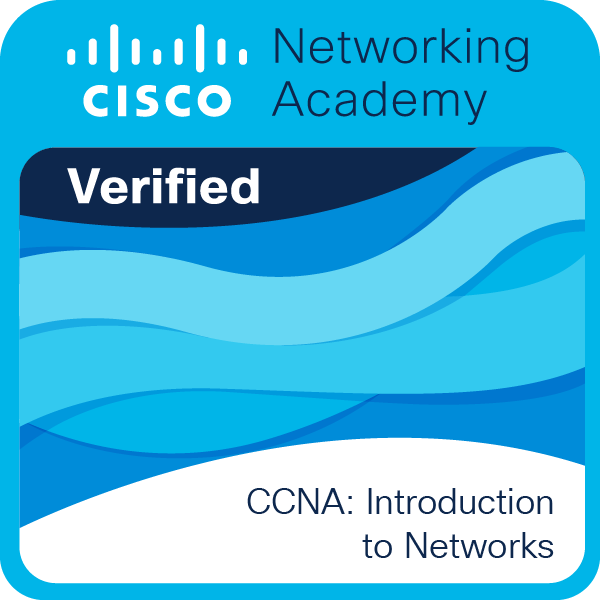
\includegraphics[width=0.75\textwidth]{../../Archivos/Imagenes_Logos/Cisco_2.png}

        \vspace{0.2cm}

       

    \end{columns}

\end{frame}


\section{Oracle Certified Professional: Java SE 17 Developer}

\begin{frame}{Oracle Certified Professional: Java SE 17 Developer}

    \begin{columns}[T]

        \column{0.65\textwidth}

        \begin{block}{Oracle Certified Professional: Java SE 17 Developer}
            \begin{itemize}
                \item Producto: Java SE 17, plataforma de desarrollo para aplicaciones empresariales y de propósito general.
                \item Empresa: Oracle Corporation es una empresa tecnológica estadounidense especializada en bases de datos, software empresarial, Java y servicios de computación en la nube.
                \item Cursos previos: Become a Java SE 17 Developer, ruta oficial de Oracle con más de 37 horas de capacitación; incluye Java SE 17 Programming y novedades de Java 17.
                \item Certificación: Oracle Certified Professional: Java SE 17 Developer (1Z0-829), examen de 90 minutos, 50 preguntas y costo publicado de US \(\mathdollar245\)
            \end{itemize} 
        \end{block}

    \end{columns}

\end{frame}


\section{Oracle}

\begin{frame}{Oracle}

       \begin{columns}[T]

        % Imagen izquierda
        \column{0.48\textwidth}
        \centering
        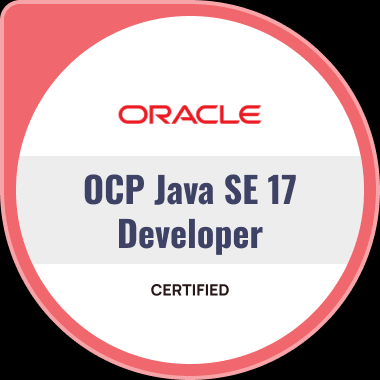
\includegraphics[width=0.75\textwidth]{../../Archivos/Imagenes_Logos/Oracle_1.png}

        \vspace{0.2cm}

        

        % Imagen derecha
        \column{0.48\textwidth}
        \centering
        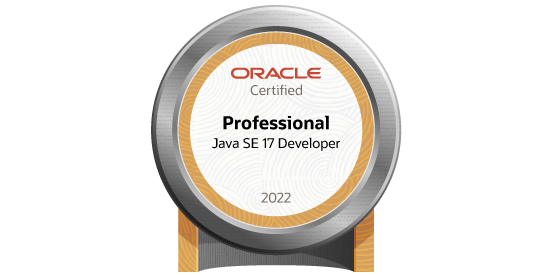
\includegraphics[width=0.75\textwidth]{../../Archivos/Imagenes_Logos/Oracle_2.png}

        \vspace{0.2cm}

       
    \end{columns}

\end{frame}


% =================================================
% REFERENCIAS
% =================================================

\section{Referencias}

\begin{frame}[allowframebreaks]{Referencias}

\begin{thebibliography}{99}

\bibitem{aws2026}
Amazon Web Services. (2026).
\textit{AWS Certified Cloud Practitioner}.
AWS Certification.
\url{https://aws.amazon.com/es/certification/certified-cloud-practitioner/}

\vspace{0.3cm}

\bibitem{cisco2026}
Cisco Systems, Inc. (2026).
\textit{Cisco Certified Network Associate (CCNA)}.
Cisco CCNA.
\url{https://www.cisco.com/site/us/en/learn/training-certifications/exams/ccna.html}

\vspace{0.3cm}

\bibitem{google2026}
Google Cloud. (2026).
\textit{Associate Cloud Engineer certification}.
Google Cloud Certification.
\url{https://cloud.google.com/learn/certification/cloud-engineer?hl=es}

\vspace{0.3cm}

\bibitem{microsoft2026}
Microsoft. (2026).
\textit{Microsoft Certified: Azure Fundamentals}.
Microsoft Learn.
\url{https://learn.microsoft.com/es-es/credentials/certifications/azure-fundamentals/}

\vspace{0.3cm}

\bibitem{oracle2026}
Oracle. (2026).
\textit{Become a Java SE 17 Developer}.
Oracle Training and Certification.
\url{https://learn.oracle.com/ols/learning-path/become-a-java-se-17-developer/88323/99487}

\end{thebibliography}

\end{frame}

\end{document}